\documentclass{beamer}

\usepackage[utf8]{inputenc}
\usepackage{minted}
\usepackage{listings}
\usepackage{graphicx}
\usepackage{xcolor}
\usepackage{adjustbox}


\usetheme{Madrid}
\useinnertheme{circles}
\definecolor{ssgreen}{HTML}{669B41}
\usecolortheme[named=ssgreen]{structure}
\setbeamertemplate{navigation symbols}{}

\AtBeginEnvironment{frame}{\setcounter{footnote}{0}}

\title[Kubernetes]{Introduction to Kubernetes}
\author[Ed MacDonald]{Ed MacDonald\\emacdonald@solutionstreet.com}
\institute[\href{https://solutionstreet.com}{SolutionStreet}]{SolutionStreet\\\href{https://solutionstreet.com}{(solutionstreet.com)}}
\date{July 2020}

\titlegraphic{ \includegraphics[width=2cm]{logo} }

\begin{document}
\frame{\titlepage}

\begin{frame}
\frametitle{What is Kubernetes?}
\begin{itemize}
    \item{A Container Orchestration Framework.}
    \item{Very well suited for Applications that scale horizontally (stateless).}
    \item{But can also accommodate portions of your infrastructure that do not scale horizontally (stateful). Don't let people tell you otherwise.}
\end{itemize}
\end{frame}

\begin{frame}
    \frametitle{How do you use it?}
    \begin{itemize}
        \item{Package your application components as containers.}
        \item{Run the containers on Kubernetes Pods.}
        \item{Let Kubernetes manage the Pods for you!}
    \end{itemize}
\end{frame}

\begin{frame}
    \frametitle{Why go through the hassle? (It can be a hassle)}
    \begin{itemize}
        \item{Kubernetes can increase or decrease the number of Pods according to traffic load.}
        \item{Kubernetes can increase or decrease the amount of compute resources according to compute load.}
        \item{Kubernetes can replace unresponsive Pods with new ones.}
    \end{itemize}
\end{frame}

\begin{frame}
    \begin{center}
        \Huge High Level Deployment Walkthrough
    \end{center}
\end{frame}

\begin{frame}
    \frametitle{Deploying An App: Build Your App}
    \includegraphics[width=\textwidth,height=0.85\textheight,keepaspectratio]{graphics/deploy-00-app.eps}
\end{frame}

\begin{frame}
    \frametitle{Deploying An App: Package Your App as a Container}
    \includegraphics[width=\textwidth,height=0.85\textheight,keepaspectratio]{graphics/deploy-01-appContainerized.eps}
\end{frame}

\begin{frame}
    \frametitle{Deploying An App: Push The Container to a Repository}
    \includegraphics[width=\textwidth,height=0.85\textheight,keepaspectratio]{graphics/deploy-02-containerToRepo.eps}
\end{frame}

\begin{frame}
    \frametitle{Deploying An App: Deploy Pods to a Kubernetes Cluster}
    \includegraphics[width=\textwidth,height=0.85\textheight,keepaspectratio]{graphics/deploy-03-emptyPods.eps}
\end{frame}

\begin{frame}
    \frametitle{Deploying An App: Pods Pull Your Container}
    \includegraphics[width=\textwidth,height=0.85\textheight,keepaspectratio]{graphics/deploy-04-podsWithContainers.eps}
\end{frame}

\begin{frame}
    \begin{center}
        \Huge Simple, right? Now let's get into the weeds.
    \end{center}
\end{frame}

\begin{frame}
    \frametitle{Kubernetes Nodes}
    \begin{itemize}
        \item The (virtual) machines that make up the Kubernetes Cluster.
        \item Kubernetes schedules Pods to run on these Nodes.
        \item Kubernetes changes the number of Nodes to increase/decrease compute resources.
    \end{itemize}
\end{frame}

\begin{frame}
    \frametitle{Tool: minikube\footnotemark}
    \begin{itemize}
        \item Easiest way to install a (single node) Kubernetes cluster on your machine.
        \item For development purposes only!
    \end{itemize}
    \footnotetext[1]{https://kubernetes.io/docs/tasks/tools/install-minikube}
\end{frame}

% https://www.patrickbaylis.com/posts/2018-10-11-beamer-resizing/
\begin{frame}
    \frametitle{Kubernetes Nodes}
    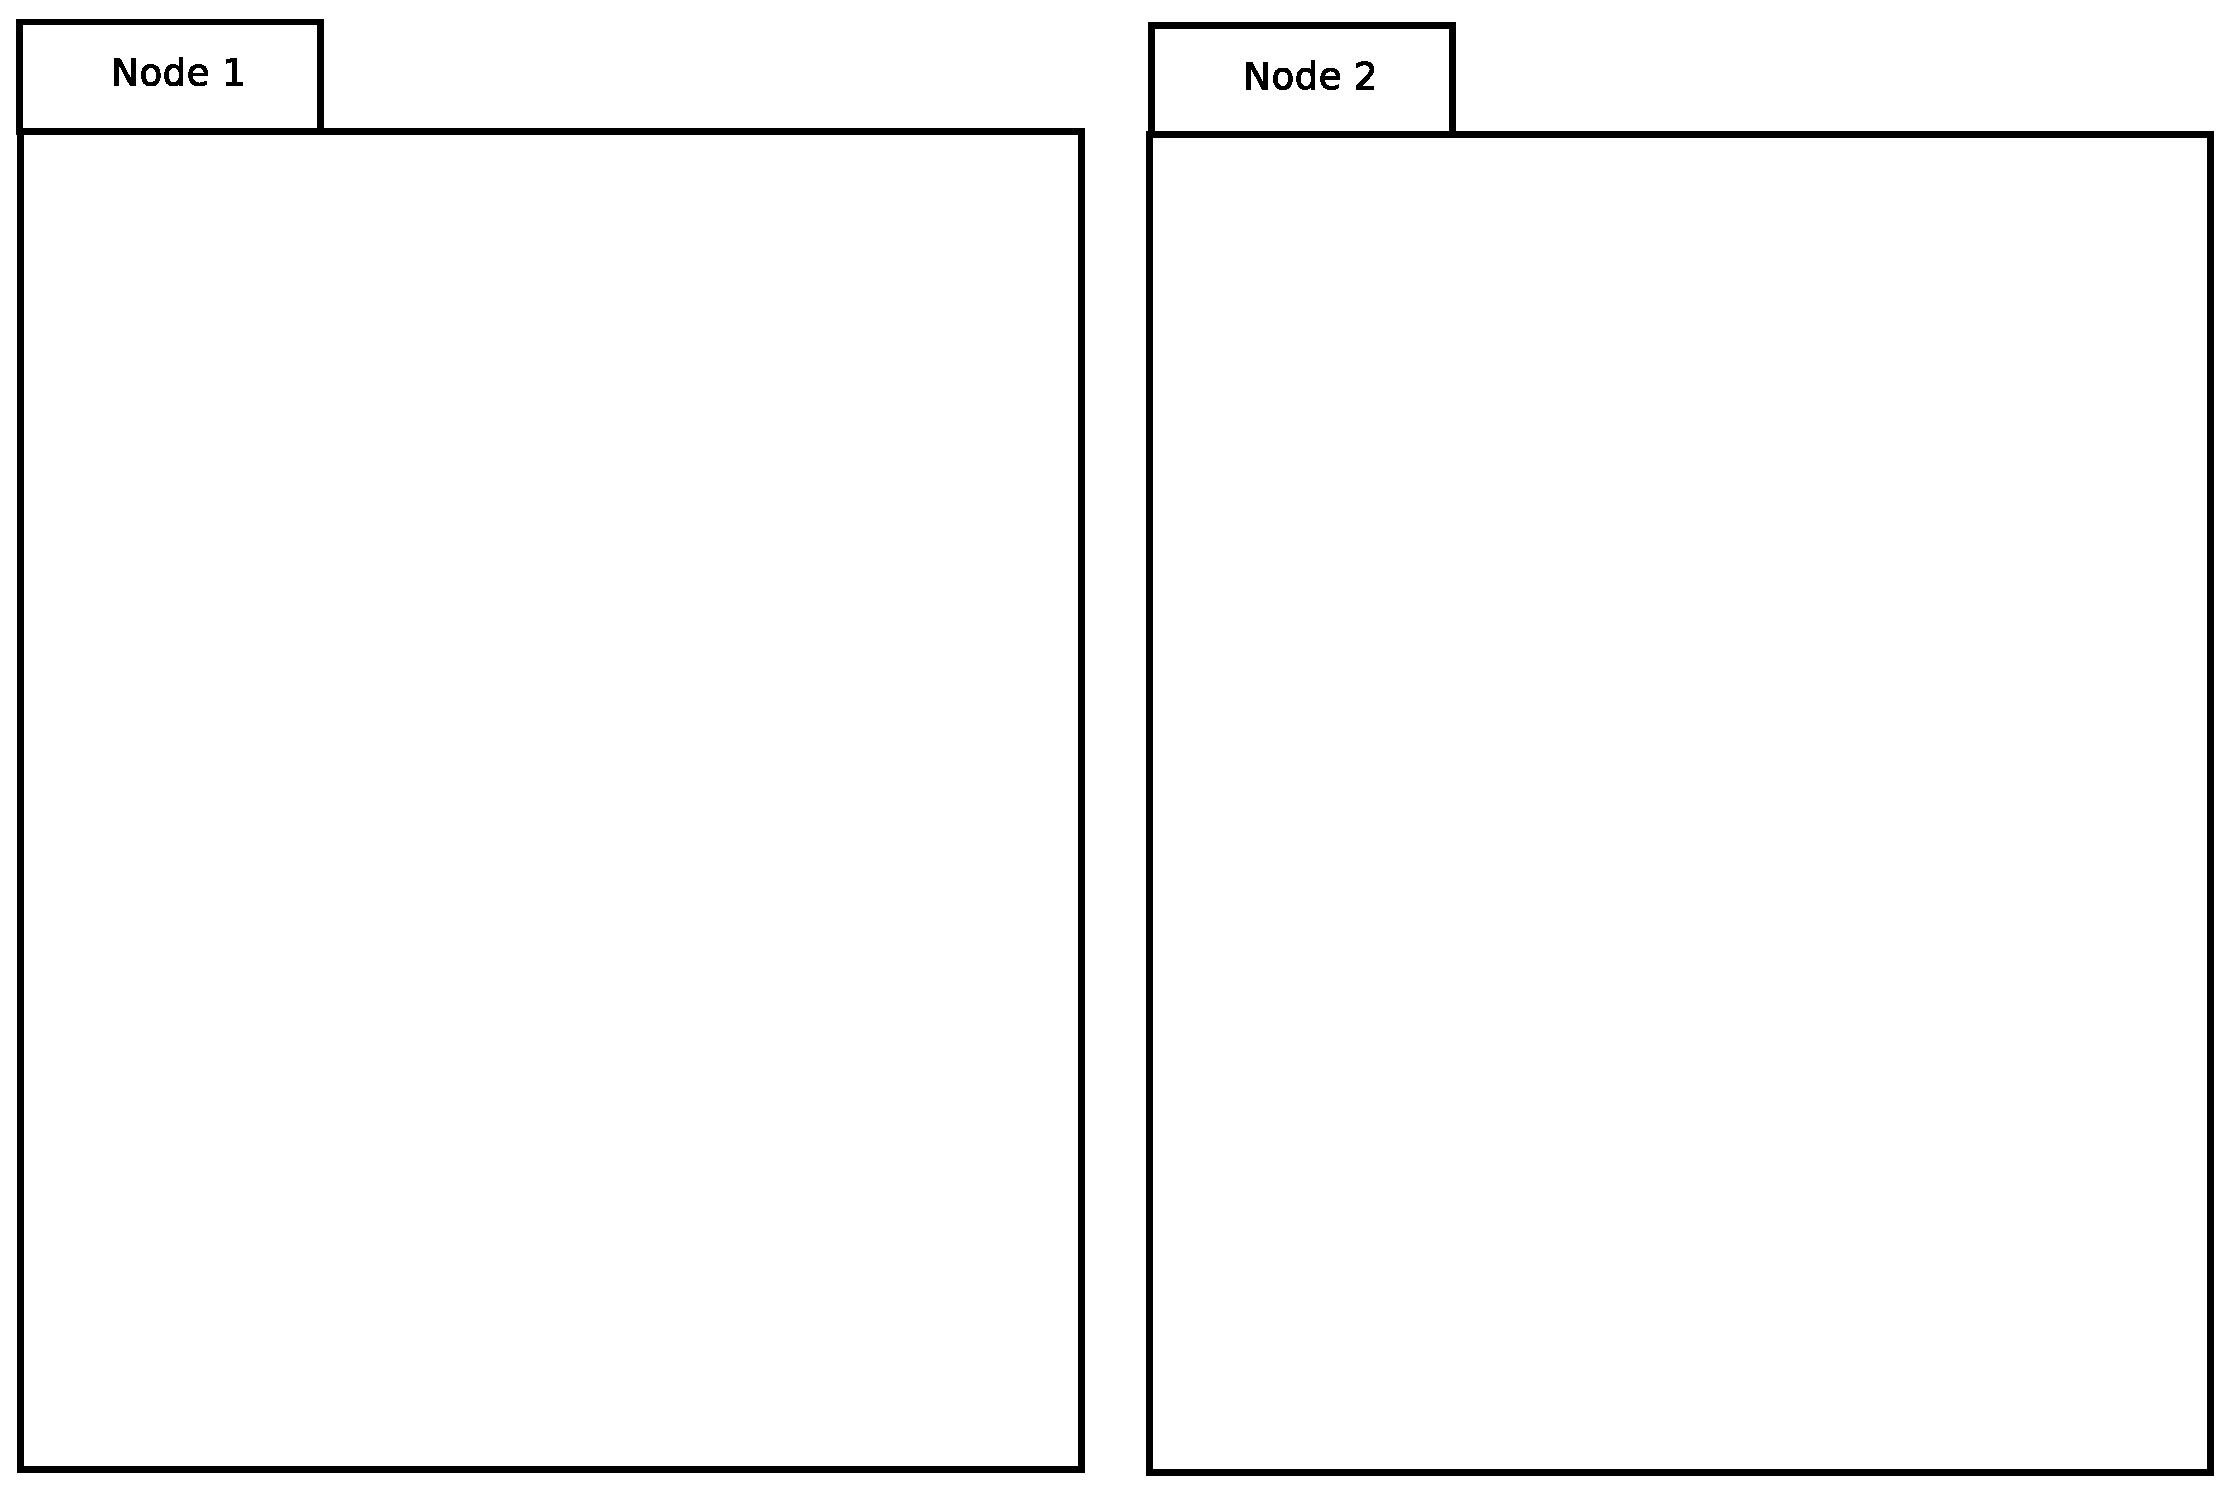
\includegraphics[width=\textwidth,height=0.85\textheight,keepaspectratio]{graphics/00-nodes.eps}
\end{frame}

\begin{frame}
    \frametitle{Pods}
    Pods (not containers!) are the fundamental building blocks of a Kubernetes application
    \begin{itemize}
        \item A Pod is a group of one or more containers that work closely together on a specific task.
        \item Pods manage Volumes for their Containers.
        \item Pods specify health check endpoints for their Containers.
        \item Kubernetes software is deployed as Pods on the Cluster!
    \end{itemize}
\end{frame}

\begin{frame}
    \frametitle{System Pods}
    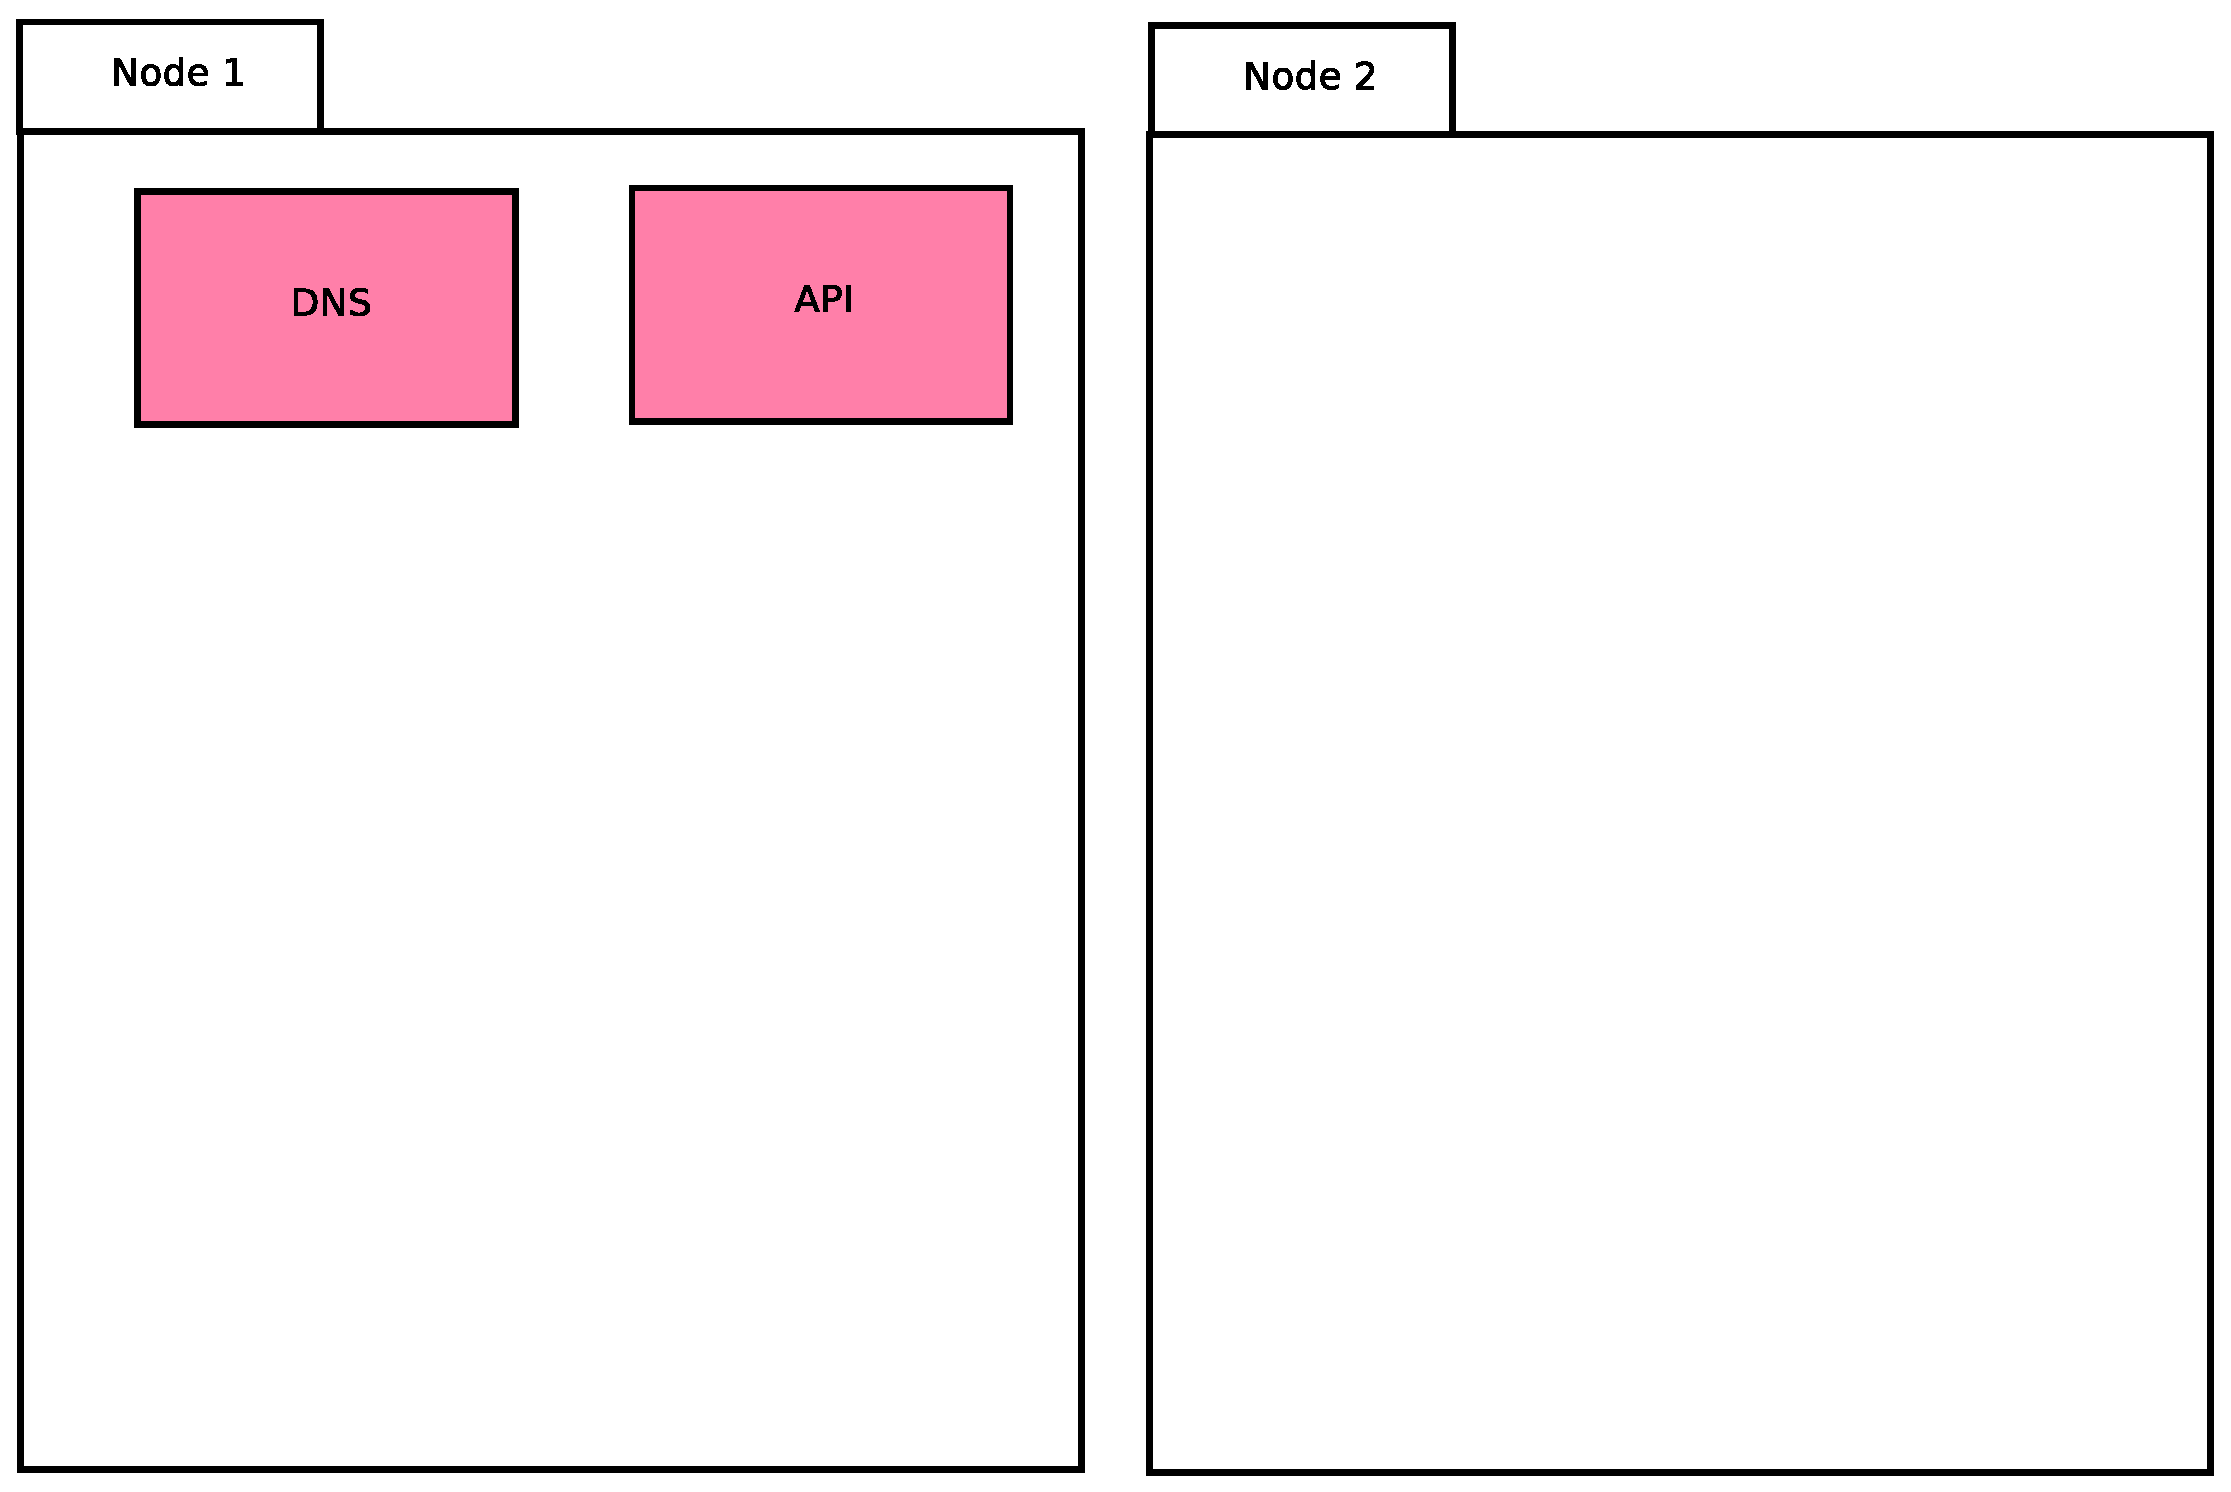
\includegraphics[width=\textwidth,height=0.85\textheight,keepaspectratio]{graphics/01-systemPods.eps}
\end{frame}

\begin{frame}
    \frametitle{The Sample Apps}
    I wrote two apps that do nothing other than suggest a random Subreddit.
    \begin{itemize}
        \item One is stateless and selects at random from a list of 280 Subreddits.
        \begin{itemize}
            \item The list never changes.
            \item It doesn't need to store anything anywhere.
        \end{itemize}
        \item One is stateful and removes each Subreddit from the list upon suggesting it.
        \begin{itemize}
            \item It removes the selected Subreddit from the list.
            \item Persists the list.
            \item Uses the updated list to service the next request.
        \end{itemize}
    \end{itemize}
\end{frame}

\begin{frame}
    \frametitle{Tool: docker\footnotemark}
    \begin{itemize}
        \item Our apps need to be packaged as Docker Containers.
        \item We need to be able to build our Containers and publish them to minikube's docker server.
    \end{itemize}
    \footnotetext[1]{https://www.docker.com/get-started}
\end{frame}

\begin{frame}
    \frametitle{An Aside on Pods}
    \begin{itemize}
        \item Pods come and go.
        \begin{itemize}
            \item They can be replaced if unresponsive.
            \item They can be deleted on one Node and added on another (moved).
            \item \textbf{You cannot prevent either of these things from happening.}
        \end{itemize}
        \item By default, when Pods are replaced or moved, the volumes they get won't be the ones they had before.
        \item By default, they'll also have new hostnames.
        \item Not a big deal for stateless Applications.
        \item Definitely something that needs to be addressed for our stateful Application, though.
    \end{itemize}
\end{frame}

\begin{frame}
    \frametitle{Stateless Application Pods}
    \includegraphics[width=\textwidth,height=0.85\textheight,keepaspectratio]{graphics/02-statelessAppPods.eps}
\end{frame}

\begin{frame}
    \frametitle{Stateful Application Pods}
    \includegraphics[width=\textwidth,height=0.85\textheight,keepaspectratio]{graphics/03-statefulAppPods.eps}
\end{frame}

\begin{frame}
    \frametitle{Controllers}
    \begin{itemize}
        \item Don't create Pods directly.
        \item Instead, create a Controller that manages the Pods for you.
    \end{itemize}
\end{frame}

\begin{frame}
    \frametitle{Controllers: ReplicaSets}
    \begin{itemize}
        \item ReplicaSets allow you to declare to Kubernetes how many of a given type of Pod you wish to have running.
        \item Pods in a ReplicaSet are treated as if they are Stateless.
        \item Any Pod is indistinguishable from another from the Application's point of view.
    \end{itemize}
\end{frame}

\begin{frame}
    \frametitle{Controllers: Deployments}
    \begin{itemize}
        \item Deployments are an even higher level abstraction than Replica Sets.
        \item They provide "declarative updates to Pods", as well as other features?
        \item I use them in my example, but I don't use any features that distinguish them from ReplicaSets.
    \end{itemize}
\end{frame}

\begin{frame}
    \frametitle{Controllers: Stateful Sets}
    StatefulSets manage Pods that are required to have state, namely:
    \begin{itemize}
        \item Pods in a StatefulSet each have a persistent network identity.
        \item Pods in a StatefulSet each have persistent storage.
        \item Persistent here means they stay the same when Pods are replaced or moved. You can stop worrying about our stateful app now.
    \end{itemize}
\end{frame}

\begin{frame}
\frametitle{Tool: kubectl\footnotemark}
\begin{itemize}
\item We need to be able to communicate with our Cluster.
\item kbuectl can update components in our cluster.
\item kbuectl can inspect components in our cluster.
\item kbuectl can create components in our cluster, but we'll use another tool for that...
\end{itemize}
\footnotetext[1]{https://kubernetes.io/docs/tasks/tools/install-kubectl}
\end{frame}

\begin{frame}
\frametitle{Tool: helm\footnotemark}
\begin{itemize}
    \item Tool for packaging and deploying Kubernetes apps.
    \item We'll use helm to package and deploy our Kubernetes component specifications.
\end{itemize}
\footnotetext[1]{\href{https://helm.sh}{https://helm.sh}}
\end{frame}

\begin{frame}
    \frametitle{Deployment}
    \includegraphics[width=\textwidth,height=0.85\textheight,keepaspectratio]{graphics/04-deployment.eps}
\end{frame}

\begin{frame}
    \frametitle{StatefulSet}
    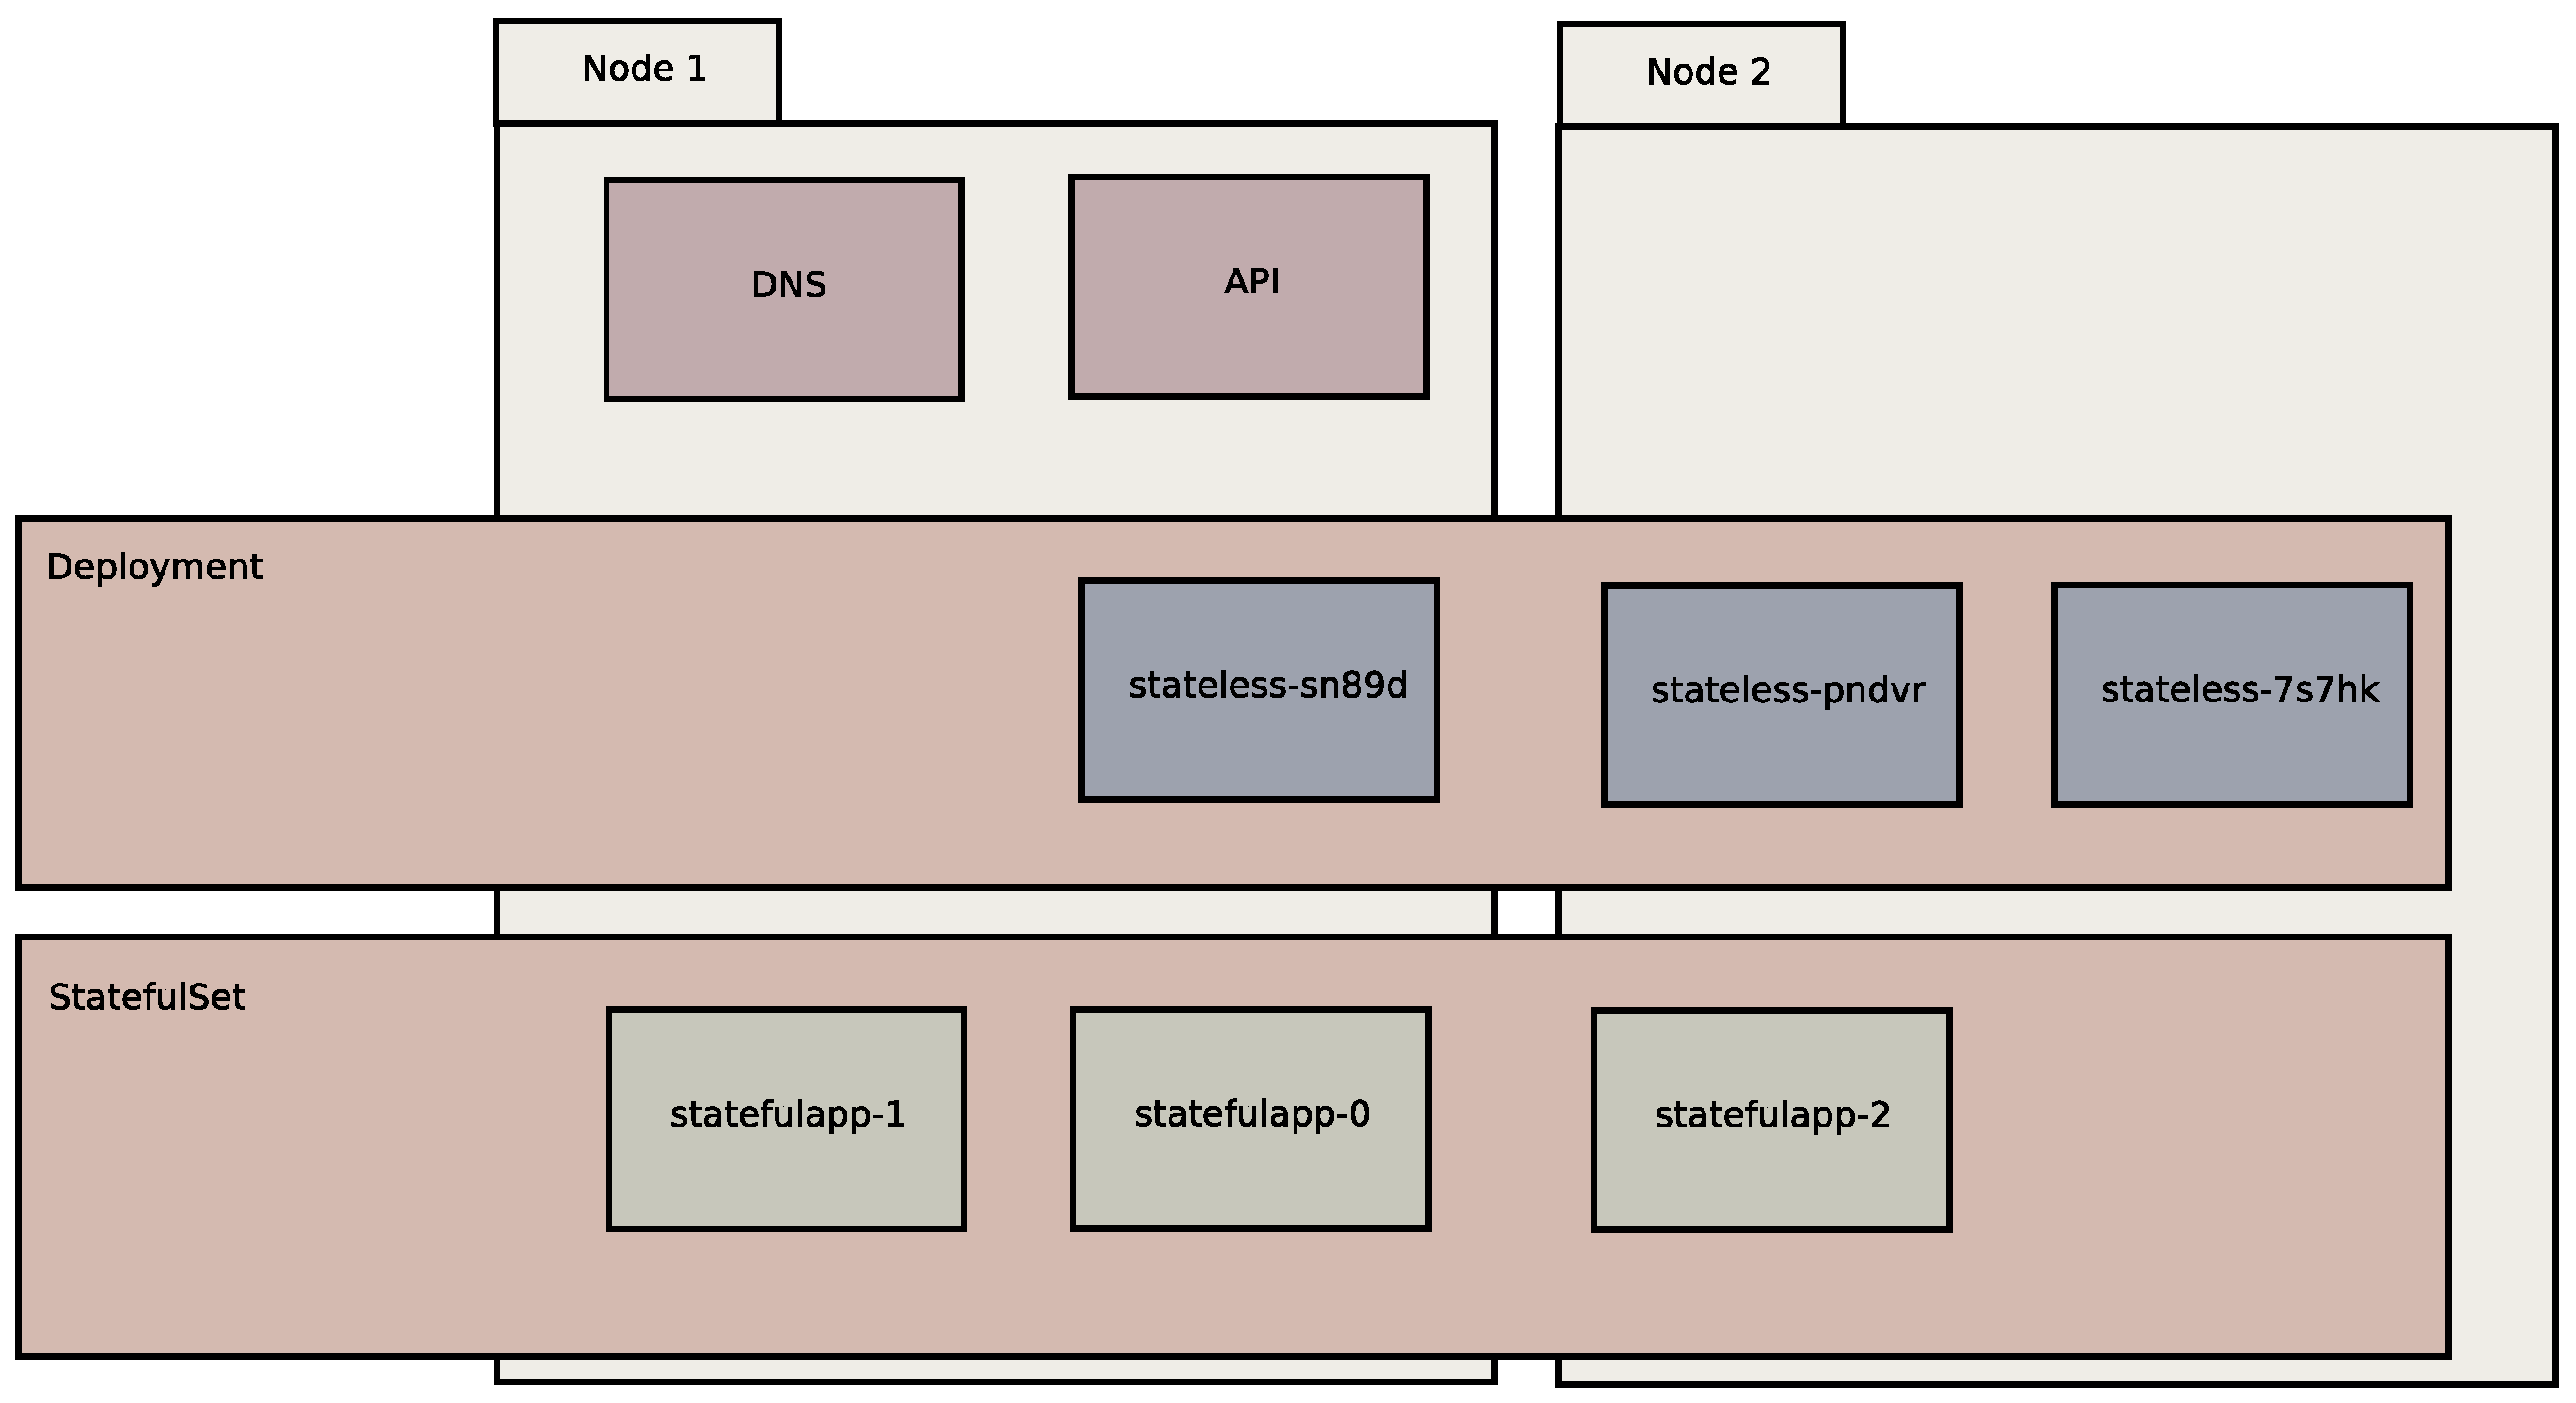
\includegraphics[width=\textwidth,height=0.85\textheight,keepaspectratio]{graphics/05-statefulSet.eps}
\end{frame}

\begin{frame}
    \frametitle{StatefulSet: Persistent Storage}
    \begin{itemize}
        \item StatefulSet pod specifications allow you to create PersistentVolumeClaims.
        \item PVCs are used to request PersistentVolumes.
        \item PersistentVolumes are volumes that survive Pods being moved or replaced.
    \end{itemize}
\end{frame}

\begin{frame}
    \frametitle{StatefulSet: Persistent Storage}
    \includegraphics[width=\textwidth,height=0.85\textheight,keepaspectratio]{graphics/06-persistence.eps}
\end{frame}

\begin{frame}
    \frametitle{StatefulSet: Headless Service}
    StatefulSets require a Headless Service
    \begin{itemize}
        \item A Headless Service is one without an IP address.
        \item It's used by the Kubernetes DNS Pod.
        \item It's what gives Pods in a StatefulSet a persistent network identity.
    \end{itemize}
\end{frame}

\begin{frame}
    \frametitle{StatefulSet: Headless Service}
    \includegraphics[width=\textwidth,height=0.85\textheight,keepaspectratio]{graphics/07-persistentIdentity.eps}
\end{frame}

\begin{frame}
    \frametitle{Load Balancers}
    \begin{itemize}
        \item Load Balancers have a "ClusterIP" and also an External IP.
        \item They balance requests sent to either IP address to all pods their "selector" targets.
    \end{itemize}
\end{frame}

\begin{frame}
    \frametitle{Load Balancers}
    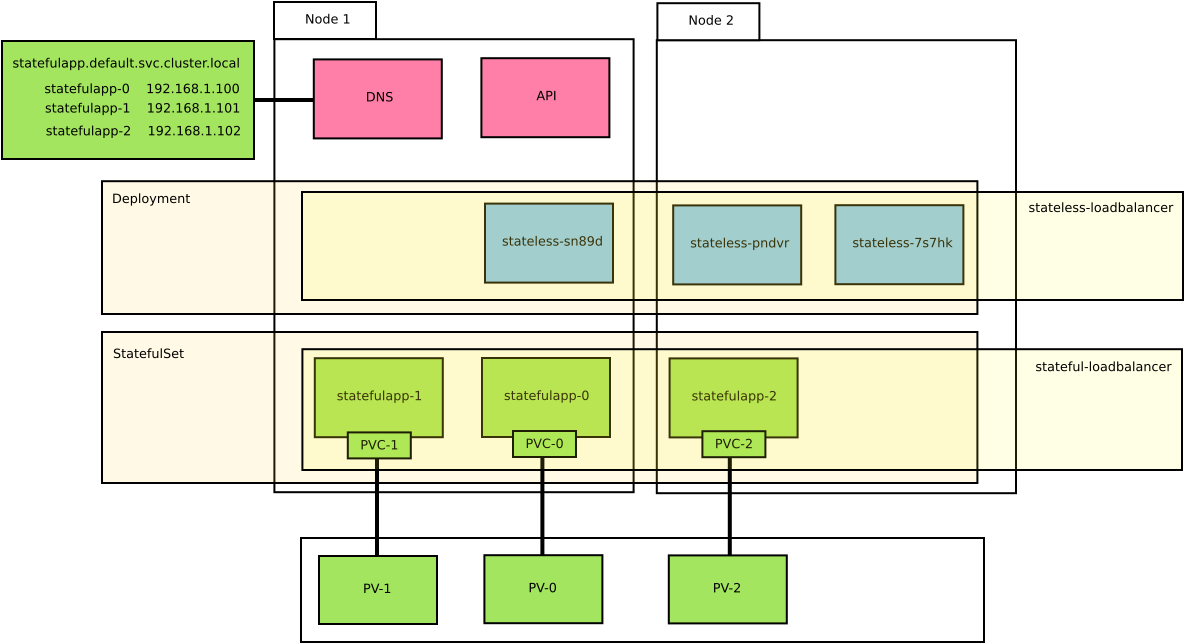
\includegraphics[width=\textwidth,height=0.85\textheight,keepaspectratio]{graphics/08-loadBalancer.eps}
\end{frame}

\begin{frame}
    \frametitle{Demo}
    \begin{center}
        \Huge So, let's see this in action!
    \end{center}
\end{frame}

\begin{frame}
    \frametitle{Overview}
    First, let's talk about the steps we're going to take:
    \begin{itemize}
        \item Start our Kubernetes environment (minikube).
        \item Configure our docker cli to talk to minikube's docker host.
        \item Build our two sample apps, package them as docker containers, and push the images.
        \item Run helm to deploy our Kubernetes components.
        \item Proxy local ports to connect to our load balancing services.
    \end{itemize}
\end{frame}

\begin{frame}
    \frametitle{Demo: Simplified Architecture}
    \includegraphics[width=\textwidth,height=0.85\textheight,keepaspectratio]{graphics/simplifiedModel-00.eps}
\end{frame}

\begin{frame}
    \begin{center}
        \Huge Time to go DEEPER?\\
        If so, let's dig into some code.
    \end{center}
\end{frame}

\begin{frame}
\frametitle{Other Resources}
Peripheral tools I used -- some of which warrant their own presentation
\begin{itemize}
    \item \LaTeX: \href{https://www.latex-project.org}{https://www.latex-project.org}
    \item Beamer: \href{https://ctan.org/pkg/beamer}{https://ctan.org/pkg/beamer}
    \item Kotlin: \href{https://kotlinlang.org}{https://kotlinlang.org}
    \item Spring Boot: \href{https://spring.io/projects/spring-boot}{https://spring.io/projects/spring-boot}
    \item Gradle: \href{https://gradle.org}{https://gradle.org}
    \item Dia: \href{http://dia-installer.de}{http://dia-installer.de}
\end{itemize}
\smallskip
Where I got my Subreddit data
\begin{itemize}
    \item Bulk Reddit data: \href{http://files.pushshift.io/reddit/subreddits}{http://files.pushshift.io/reddit/subreddits}
\end{itemize}
Finally, \textbf{\textit{this}} demo
\begin{itemize}
    \item \href{https://github.com/emacdona/k8sdemo}{https://github.com/emacdona/k8sdemo}
\end{itemize}
\end{frame}

\begin{frame}
    \begin{center}
        \Huge Questions?
    \end{center}
\end{frame}

\end{document}
